\chapter{Results} 				
% File created 28-12-2016
\label{app:appendixG-Results}



\section{Order}
\label{sec:orderApp}


\begin{figure}[H]
\centering
\subfloat[]{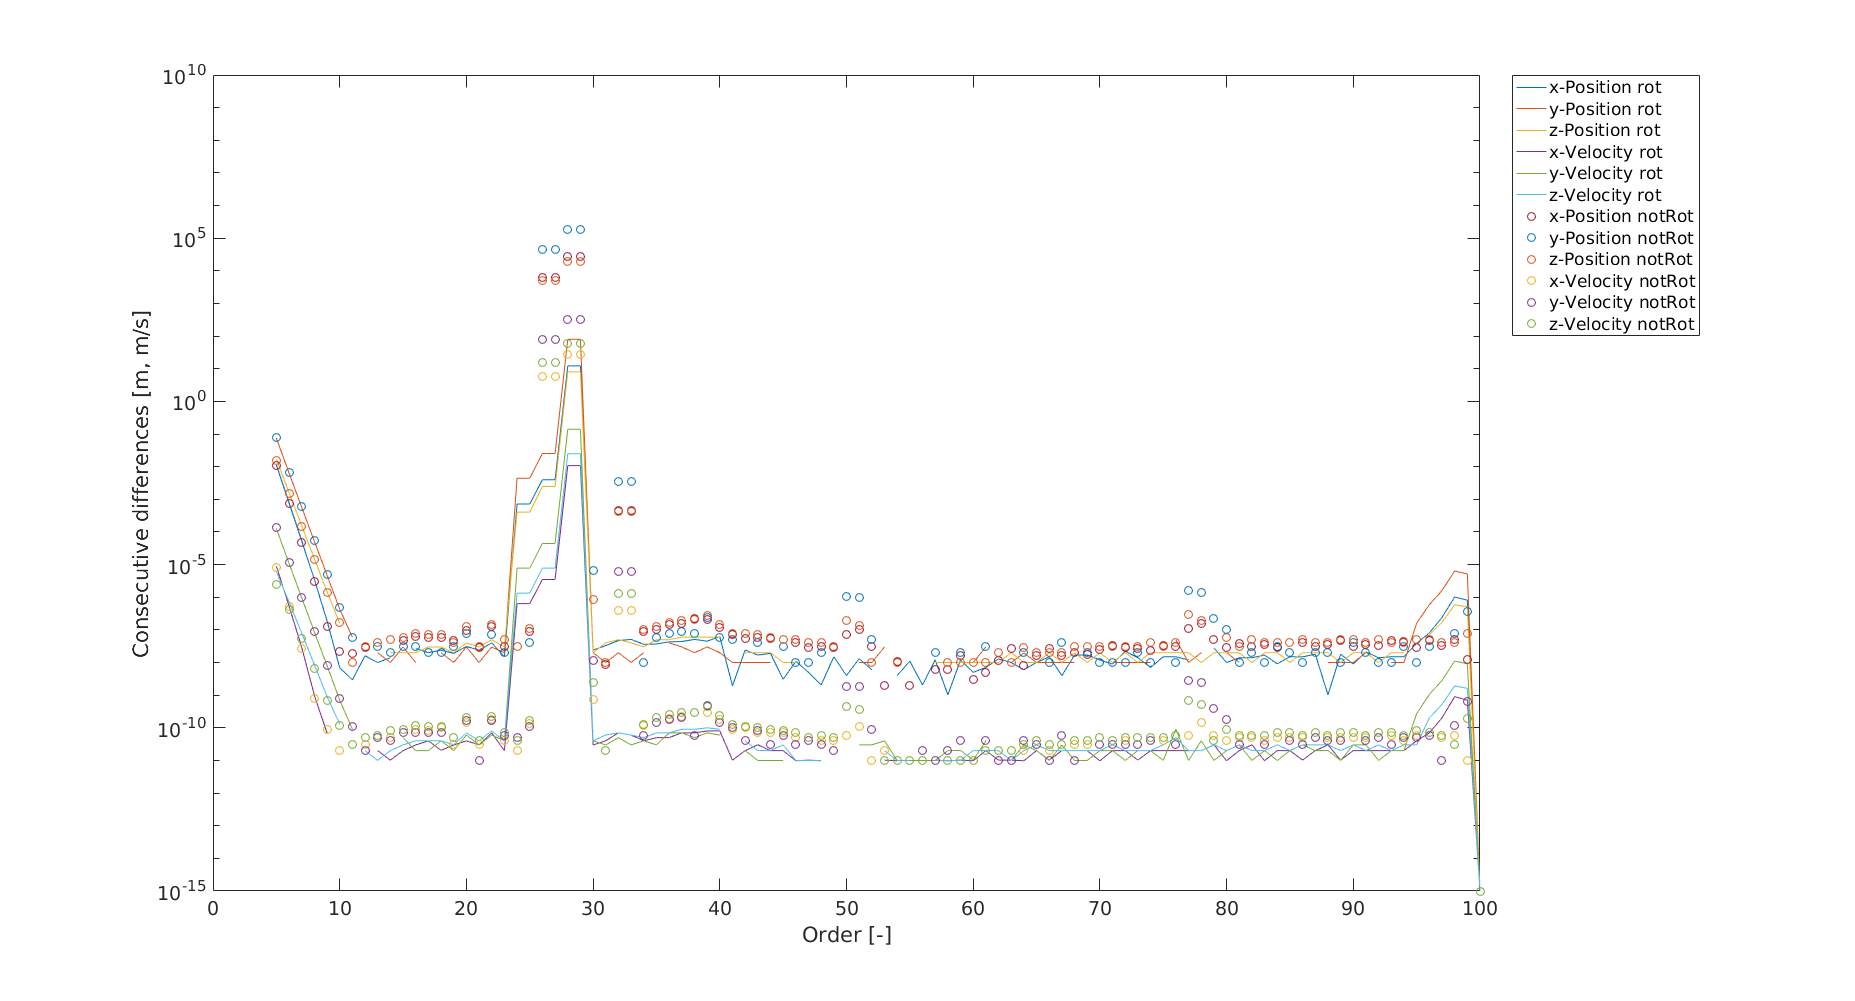
\includegraphics[width=0.8\textwidth]{figures/results/Order/orderVsConsecutiveDifferenceCase1combined.png}\label{subfig:orderVsConsecutiveDifferenceCase1combined}} \\

\subfloat[]{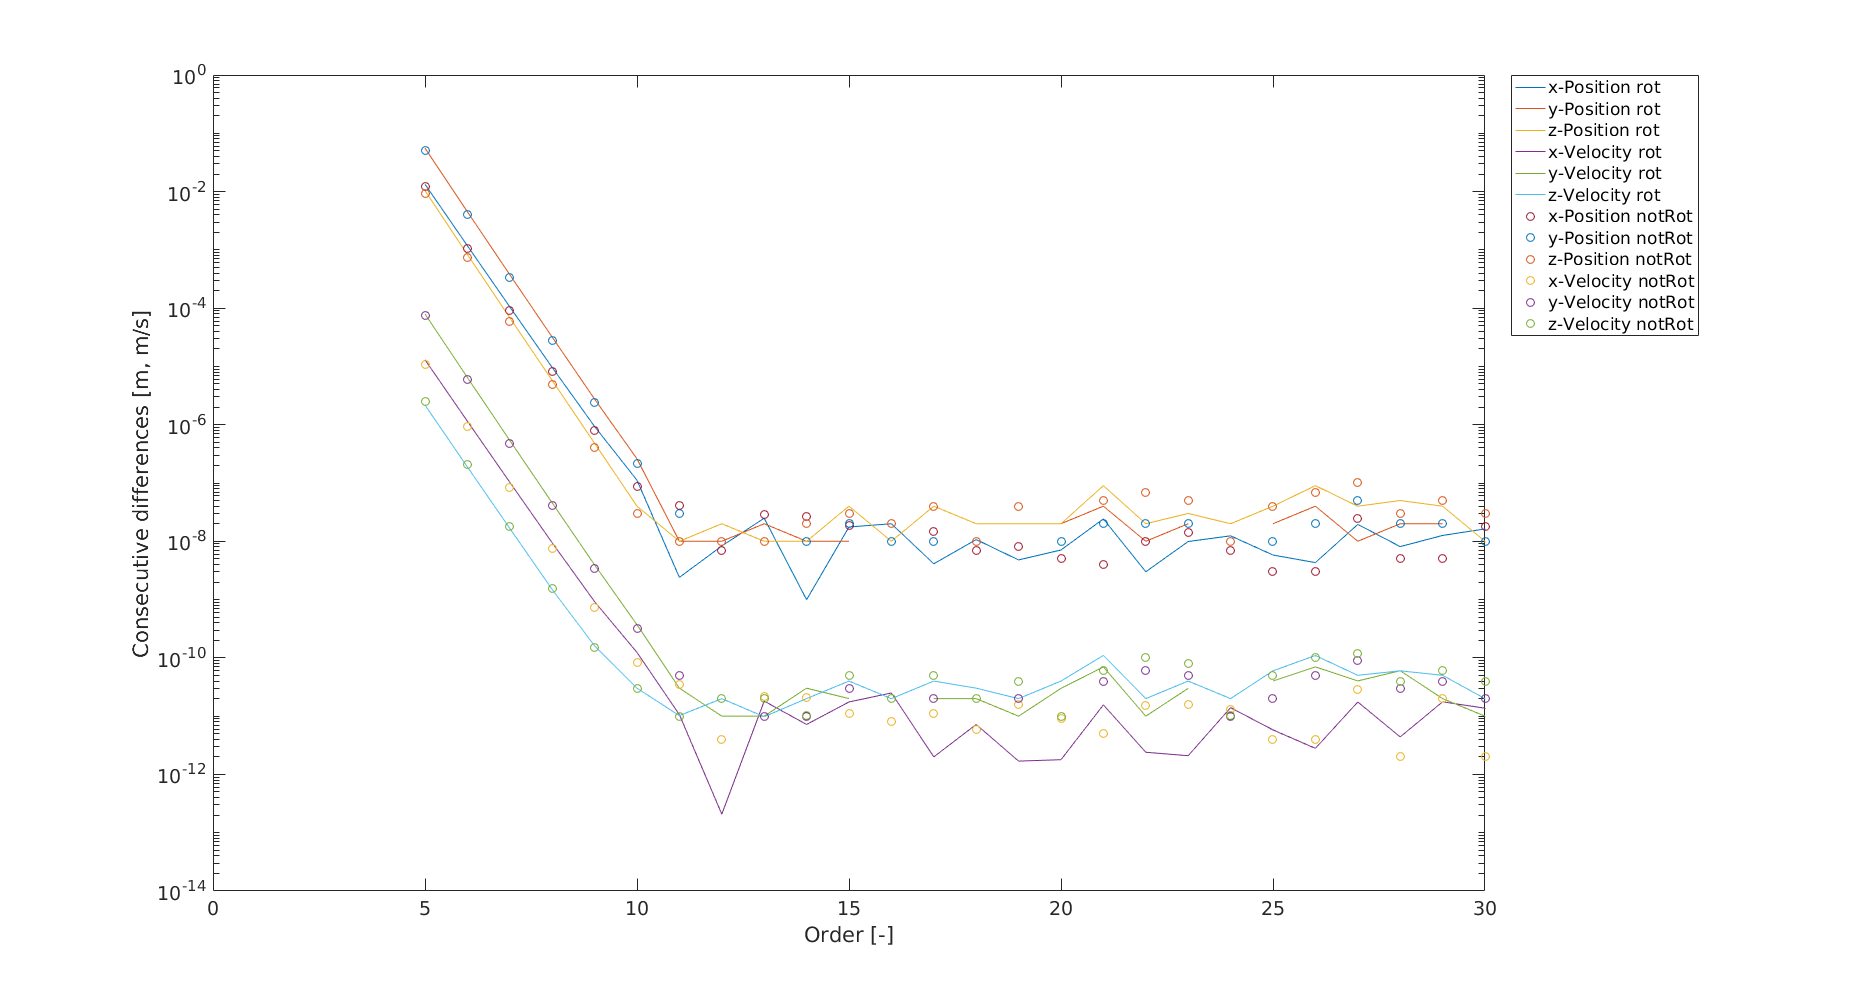
\includegraphics[width=0.8\textwidth]{figures/results/Order/orderVsConsecutiveDifferenceCase2combined.png}\label{subfig:orderVsConsecutiveDifferenceCase2combined}}
\caption{Consecutive difference for rotating and non-rotating Mars \protect\subref{subfig:orderVsConsecutiveDifferenceCase1combined} case 1, \protect\subref{subfig:orderVsConsecutiveDifferenceCase2combined} case 2 } 
\label{fig:orderVsConsecutiveDifferenceCase1combined} 
\end{figure} 

\begin{figure}[H]
\centering
\subfloat[]{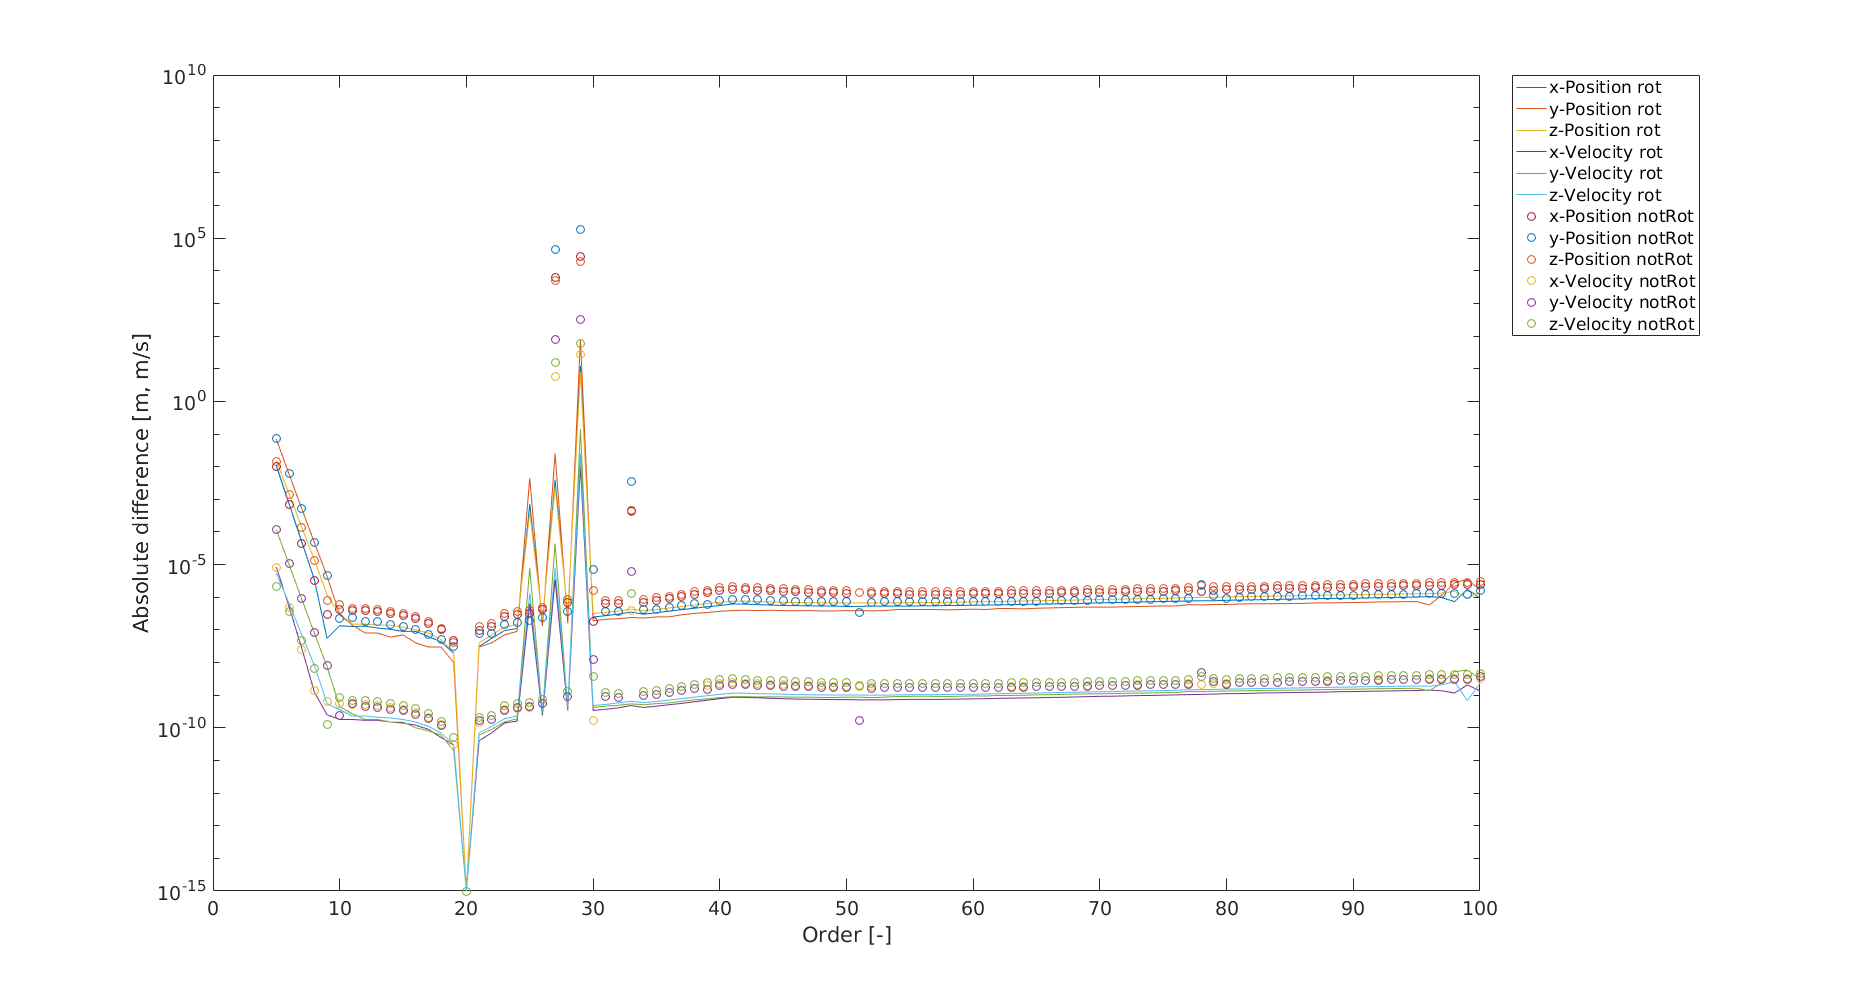
\includegraphics[width=1.2\textwidth]{figures/results/Order/orderVsNominalAbsoluteDifferenceCase1combined.png}\label{subfig:orderVsNominalAbsoluteDifferenceCase1combined}} \\

\subfloat[]{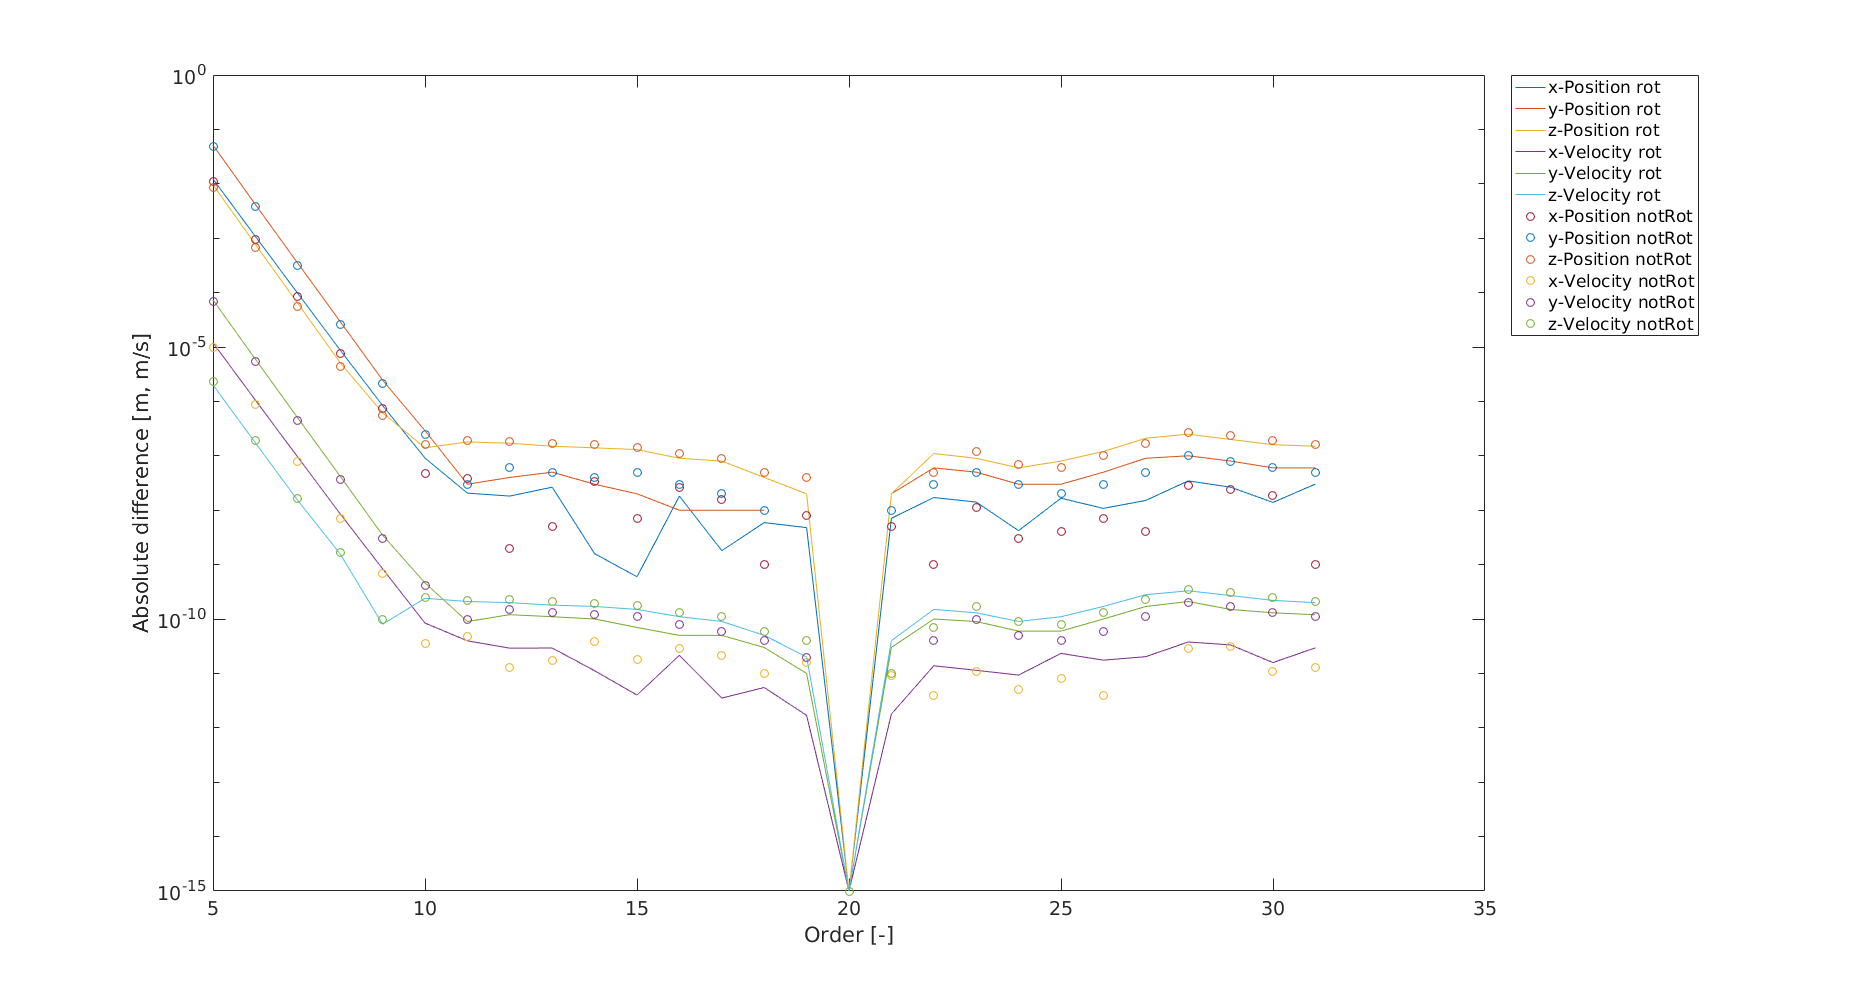
\includegraphics[width=1.2\textwidth]{figures/results/Order/orderVsNominalAbsoluteDifferenceCase2combined.png}\label{subfig:orderVsNominalAbsoluteDifferenceCase2combined}}
\caption{Difference with respect to the nominal case for rotating and non-rotating Mars \protect\subref{subfig:orderVsNominalAbsoluteDifferenceCase1combined} case 1, \protect\subref{subfig:orderVsNominalAbsoluteDifferenceCase2combined} case 2 } 
\label{fig:orderVsNominalAbsoluteDifferenceCase1combined} 
\end{figure}

%
%\section{Error tolerance}
%\label{sec:errorToleranceApp}


\section{Multiple runs}
\label{sec:multipleRunsApp}

\begin{figure}[H]
\centering
\subfloat[]{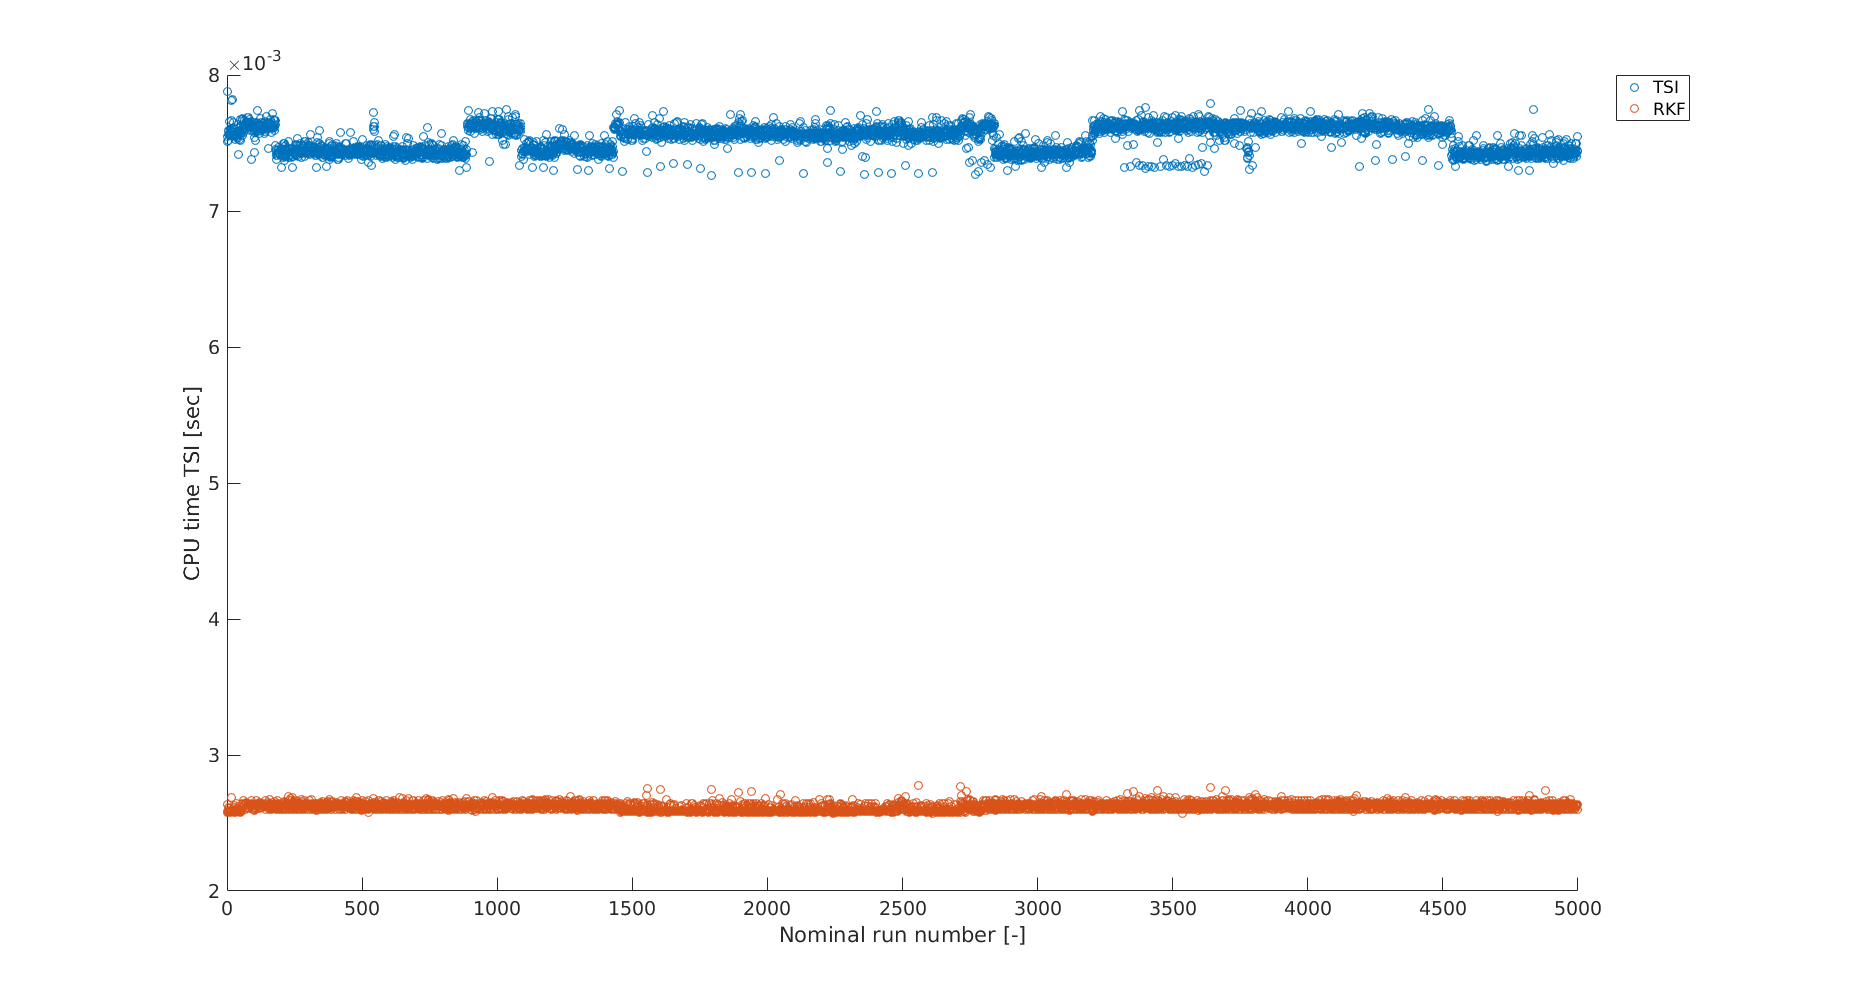
\includegraphics[width=1.2\textwidth]{figures/results/multiRun/multiRunVsCPUcase1RKFTSI.png}\label{subfig:multiRunVsCPUcase1RKFTSI}} \\

\subfloat[]{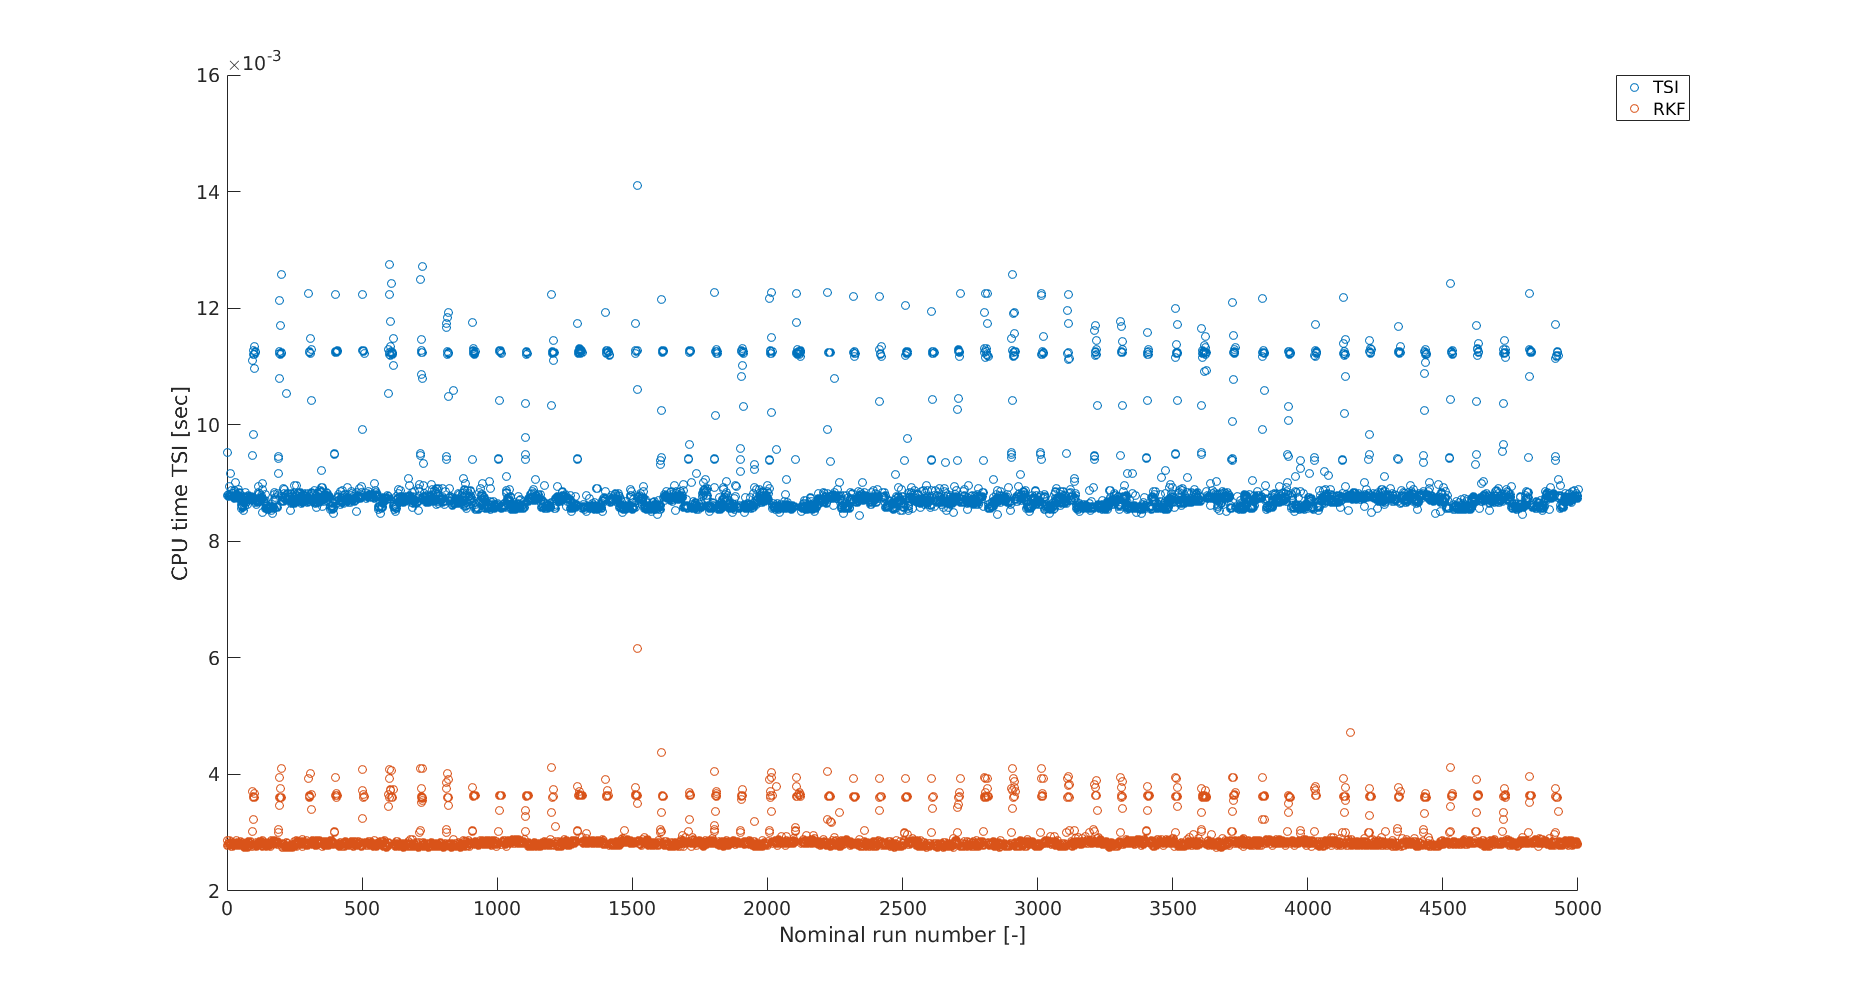
\includegraphics[width=1.2\textwidth]{figures/results/multiRun/multiRunVsCPUcase2RKFTSI.png}\label{subfig:multiRunVsCPUcase2RKFTSI}}
\caption{Nominal runs versus CPU time comparison between \ac{RKF} and \ac{TSI} \protect\subref{subfig:multiRunVsCPUcase1RKFTSI} case 1,  \protect\subref{subfig:multiRunVsCPUcase2RKFTSI} case 2 } 
\label{fig:multiRunVsCPUcase1RKFTSI} 
\end{figure} 

\begin{figure}[H]
\centering
\subfloat[]{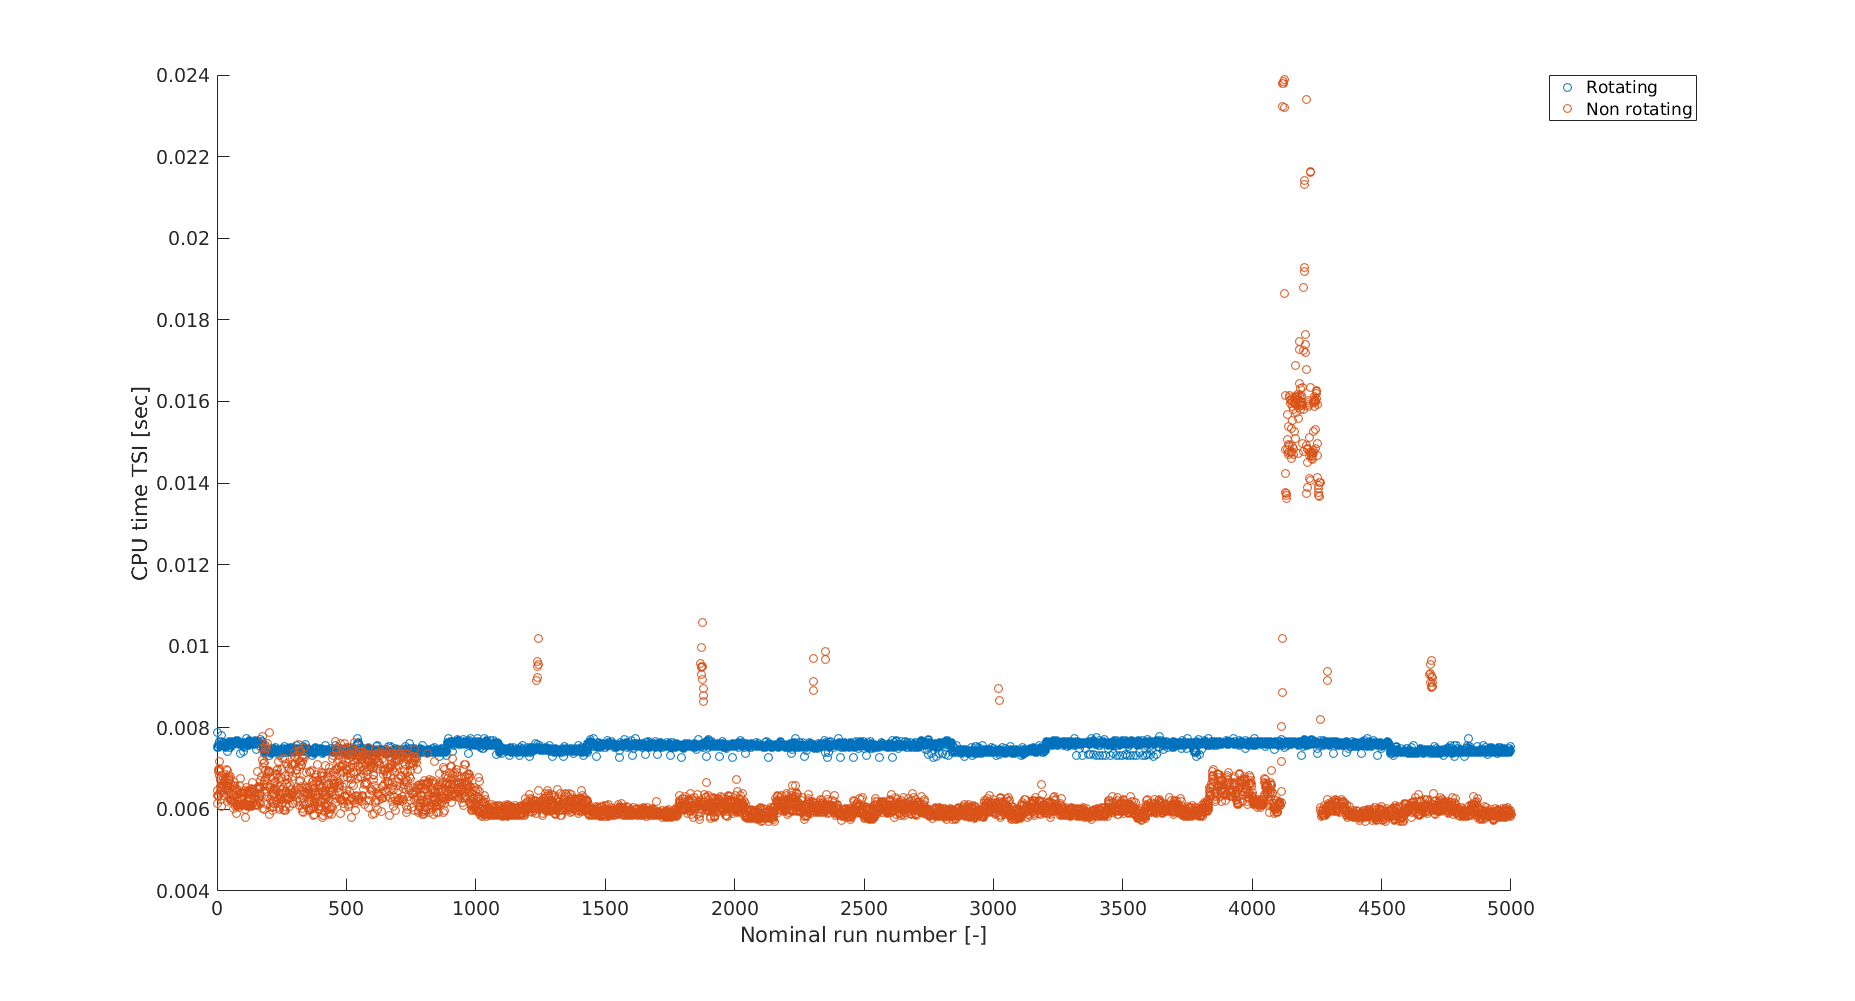
\includegraphics[width=1.2\textwidth]{figures/results/multiRun/multiRunVsCPUcase1combined.png}\label{subfig:multiRunVsCPUcase1combined}} \\

\subfloat[]{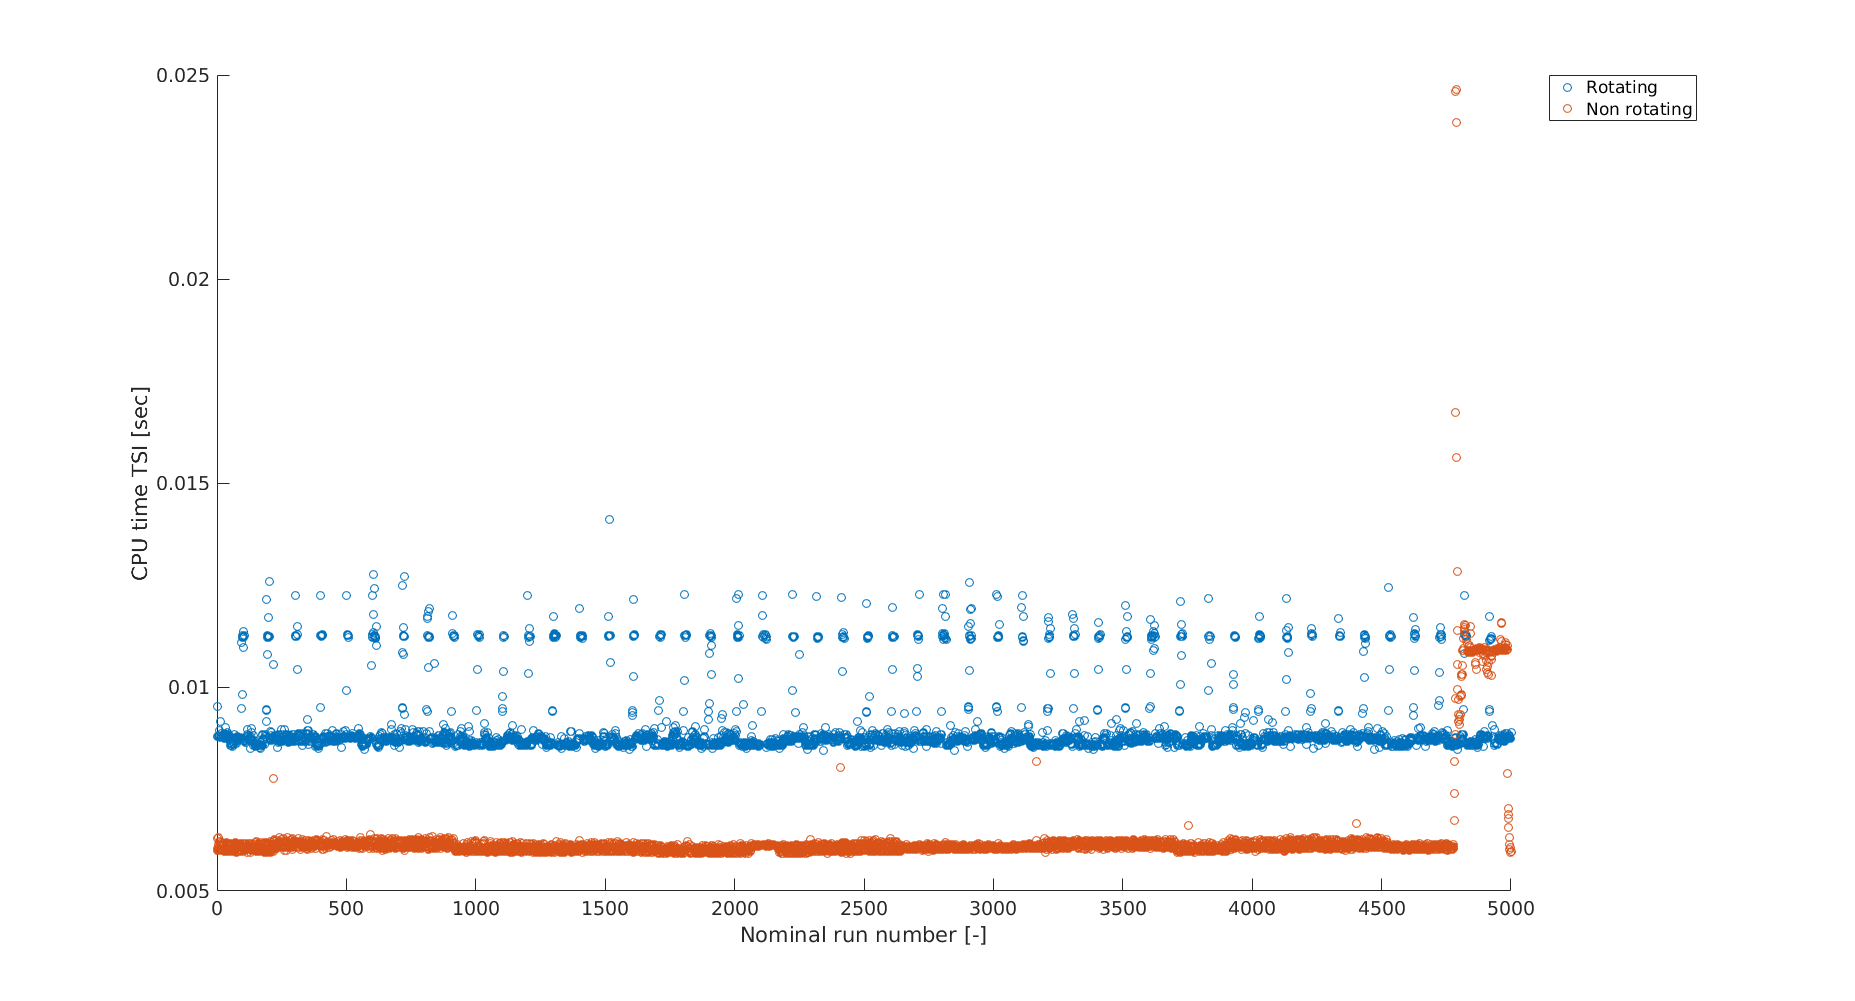
\includegraphics[width=1.2\textwidth]{figures/results/multiRun/multiRunVsCPUcase2combined.png}\label{subfig:multiRunVsCPUcase2combined}}
\caption{Nominal runs versus CPU time for rotating and non-rotating Mars \protect\subref{subfig:multiRunVsCPUcase1combined} case 1,  \protect\subref{subfig:multiRunVsCPUcase2combined} case 2 } 
\label{fig:multiRunVsCPUcase1combined} 
\end{figure} 


\section{Launch altitude}
\label{sec:launchAltitudeApp}

\begin{figure}[H]
\centering
\subfloat[]{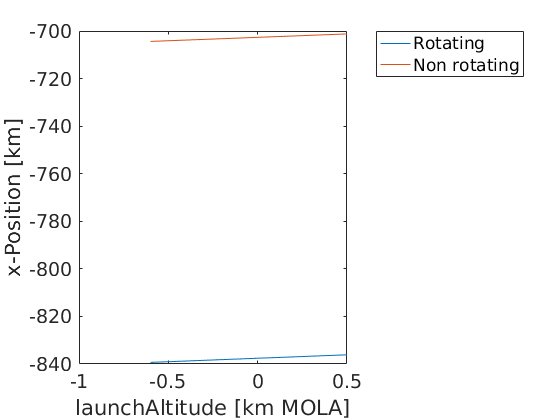
\includegraphics[scale=0.5]{figures/results/launchAltitude/launchAltitudeVsXpositionCase1combined.png}\label{subfig:launchAltitudeVsXpositionCase1combined}} 
\subfloat[]{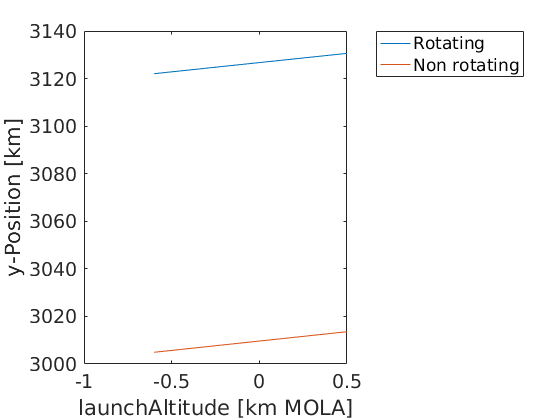
\includegraphics[scale=0.5]{figures/results/launchAltitude/launchAltitudeVsYpositionCase1combined.png}\label{subfig:launchAltitudeVsYpositionCase1combined}}
\subfloat[]{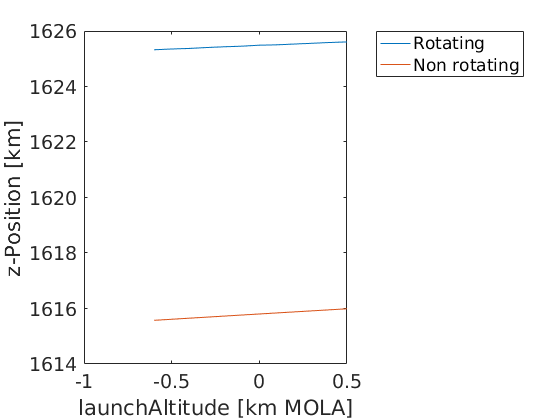
\includegraphics[scale=0.5]{figures/results/launchAltitude/launchAltitudeVsZpositionCase1combined.png}\label{subfig:launchAltitudeVsZpositionCase1combined}}\\

\subfloat[]{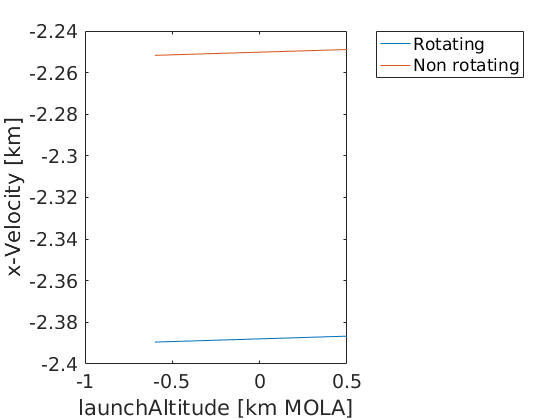
\includegraphics[scale=0.5]{figures/results/launchAltitude/launchAltitudeVsXvelocityCase1combined.png}\label{subfig:launchAltitudeVsXvelocityCase1combined}} 
\subfloat[]{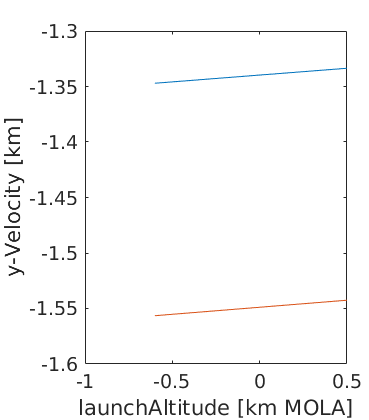
\includegraphics[scale=0.5]{figures/results/launchAltitude/launchAltitudeVsYvelocityCase1combined.png}\label{subfig:launchAltitudeVsYvelocityCase1combined}}
\subfloat[]{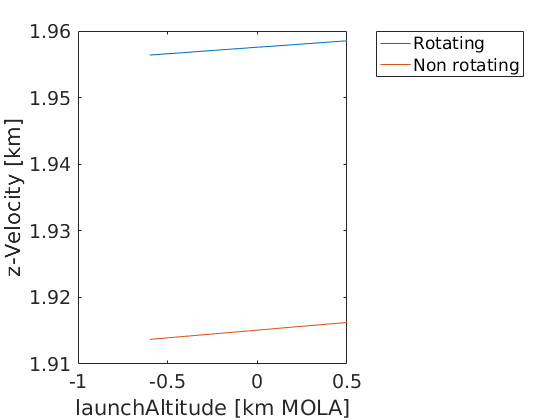
\includegraphics[scale=0.5]{figures/results/launchAltitude/launchAltitudeVsZvelocityCase1combined.png}\label{subfig:launchAltitudeVsZvelocityCase1combined}}

\caption{Launch altitude end characteristics case 1 before circularisation for rotating and non-rotating Mars \protect\subref{subfig:launchAltitudeVsXpositionCase1combined} x-position,  \protect\subref{subfig:launchAltitudeVsYpositionCase1combined} y-position,
\protect\subref{subfig:launchAltitudeVsZpositionCase1combined} z-position,  \protect\subref{subfig:launchAltitudeVsXvelocityCase1combined} x-velocity,
\protect\subref{subfig:launchAltitudeVsYvelocityCase1combined} y-velocity,  \protect\subref{subfig:launchAltitudeVsZvelocityCase1combined} z-velocity } 
\label{fig:launchAltitudeVsXpositionCase1combined} 
\end{figure} 



\begin{figure}[H]
\centering
\subfloat[]{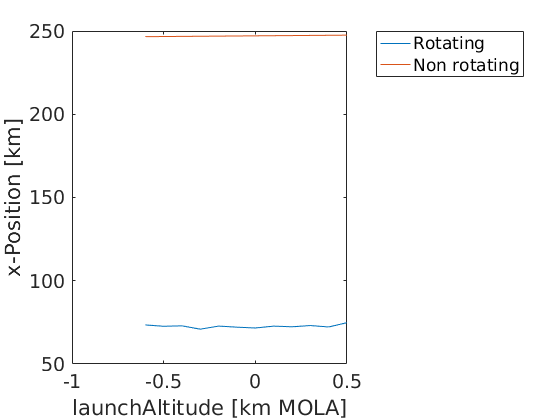
\includegraphics[scale=0.5]{figures/results/launchAltitude/launchAltitudeVsXpositionCase2combined.png}\label{subfig:launchAltitudeVsXpositionCase2combined}} 
\subfloat[]{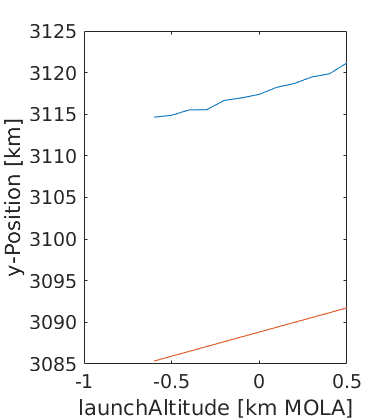
\includegraphics[scale=0.5]{figures/results/launchAltitude/launchAltitudeVsYpositionCase2combined.png}\label{subfig:launchAltitudeVsYpositionCase2combined}}
\subfloat[]{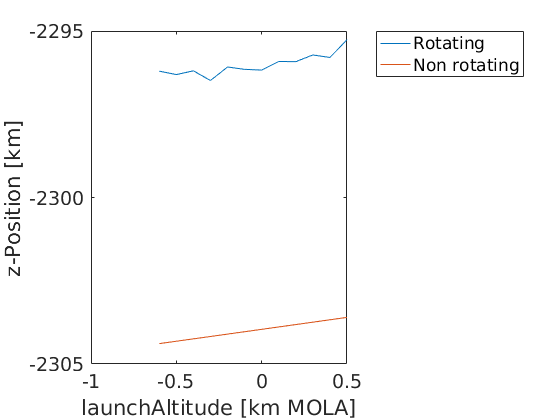
\includegraphics[scale=0.5]{figures/results/launchAltitude/launchAltitudeVsZpositionCase2combined.png}\label{subfig:launchAltitudeVsZpositionCase2combined}}\\

\subfloat[]{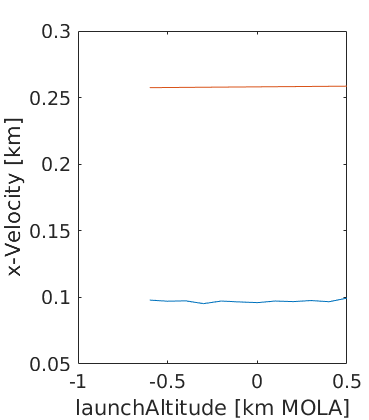
\includegraphics[scale=0.5]{figures/results/launchAltitude/launchAltitudeVsXvelocityCase2combined.png}\label{subfig:launchAltitudeVsXvelocityCase2combined}} 
\subfloat[]{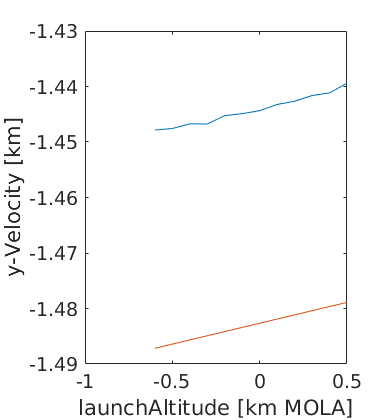
\includegraphics[scale=0.5]{figures/results/launchAltitude/launchAltitudeVsYvelocityCase2combined.png}\label{subfig:launchAltitudeVsYvelocityCase2combined}}
\subfloat[]{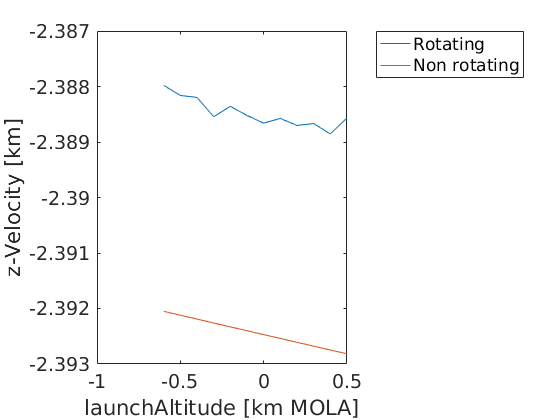
\includegraphics[scale=0.5]{figures/results/launchAltitude/launchAltitudeVsZvelocityCase2combined.png}\label{subfig:launchAltitudeVsZvelocityCase2combined}}

\caption{Launch altitude end characteristics case 2 before circularisation for rotating and non-rotating Mars \protect\subref{subfig:launchAltitudeVsXpositionCase2combined} x-position,  \protect\subref{subfig:launchAltitudeVsYpositionCase2combined} y-position,
\protect\subref{subfig:launchAltitudeVsZpositionCase2combined} z-position,  \protect\subref{subfig:launchAltitudeVsXvelocityCase2combined} x-velocity,
\protect\subref{subfig:launchAltitudeVsYvelocityCase2combined} y-velocity,  \protect\subref{subfig:launchAltitudeVsZvelocityCase2combined} z-velocity } 
\label{fig:launchAltitudeVsXpositionCase2combined} 
\end{figure} 

\begin{figure}[H]
\centering
\subfloat[]{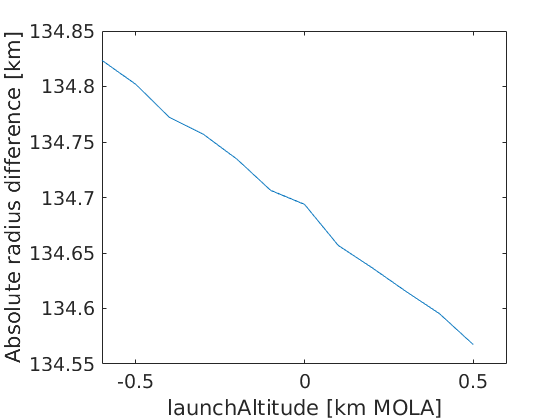
\includegraphics[width=3.1in]{figures/results/launchAltitude/launchAltitudeVsAbsRadiusDiffCase1combined.png}\label{subfig:launchAltitudeVsAbsRadiusDiffCase1combined}} 
\subfloat[]{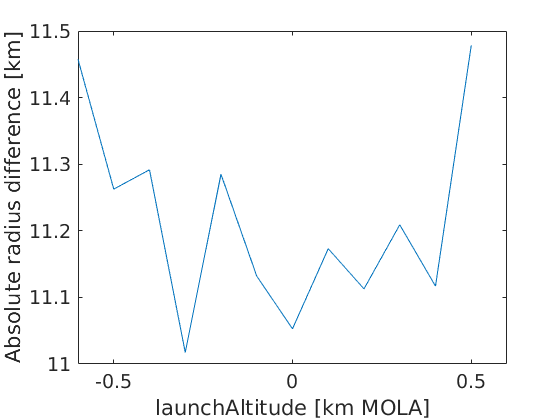
\includegraphics[width=3.1in]{figures/results/launchAltitude/launchAltitudeVsAbsRadiusDiffCase2combined.png}\label{subfig:launchAltitudeVsAbsRadiusDiffCase2combined}}
\caption{Launch altitude versus radius difference between a rotating and a non-rotating Mars \protect\subref{subfig:launchAltitudeVsAbsRadiusDiffCase1combined} case 1,  \protect\subref{subfig:launchAltitudeVsAbsRadiusDiffCase2combined} case 2 } 
\label{fig:launchAltitudeVsAbsRadiusDiffCase1combined} 
\end{figure} 

\begin{figure}[H]
\centering
\subfloat[]{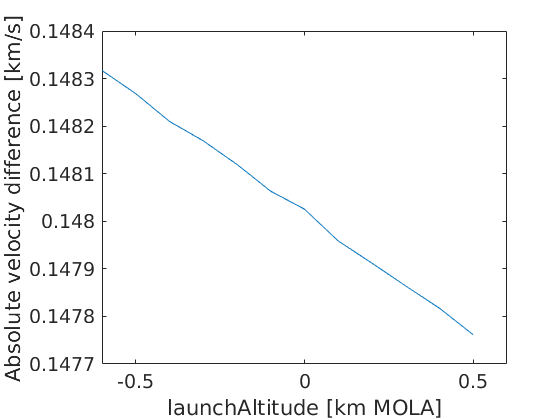
\includegraphics[width=3.1in]{figures/results/launchAltitude/launchAltitudeVsAbsVGdiffCase1combined.png}\label{subfig:launchAltitudeVsAbsVGdiffCase1combined}} 
\subfloat[]{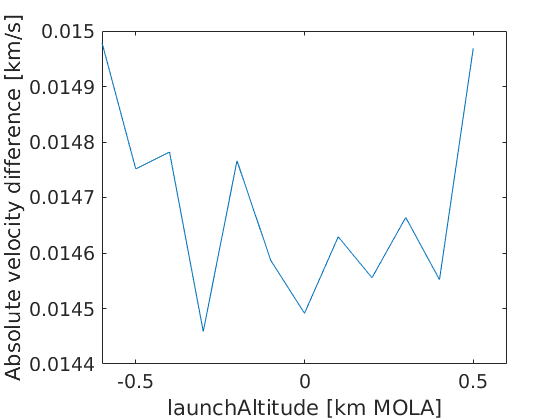
\includegraphics[width=3.1in]{figures/results/launchAltitude/launchAltitudeVsAbsVGdiffCase2combined.png}\label{subfig:launchAltitudeVsAbsVGdiffCase2combined}}
\caption{Launch altitude versus velocity difference between a rotating and a non-rotating Mars \protect\subref{subfig:launchAltitudeVsAbsVGdiffCase1combined} case 1,  \protect\subref{subfig:launchAltitudeVsAbsVGdiffCase2combined} case 2 } 
\label{fig:launchAltitudeVsAbsVGdiffCase1combined} 
\end{figure}

\section{Launch latitude}
\label{sec:launchLatitudeApp}



\begin{figure}[H]
\centering
\subfloat[]{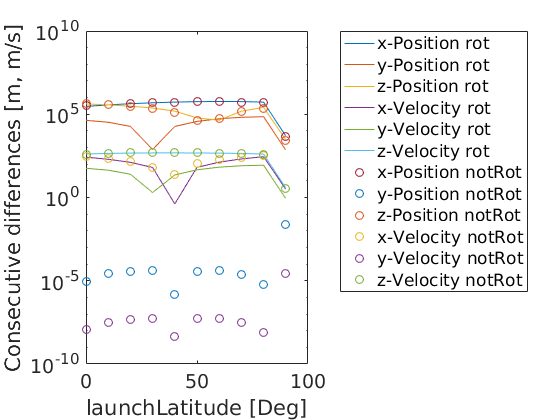
\includegraphics[width=3.1in]{figures/results/launchLatitude/launchLatitudeVsConsecutiveDifferenceCase1combinedSmall.png}\label{subfig:launchLatitudeVsConsecutiveDifferenceCase1combinedSmall}} 
\subfloat[]{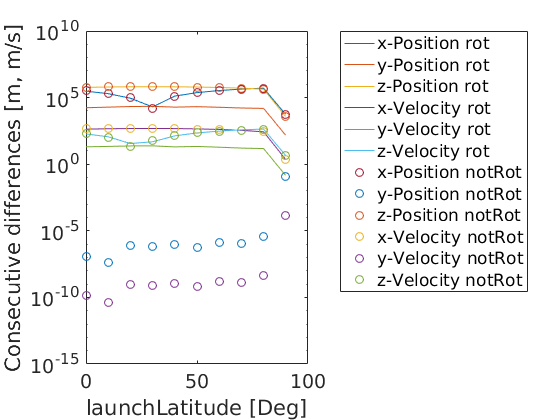
\includegraphics[width=3.1in]{figures/results/launchLatitude/launchLatitudeVsConsecutiveDifferenceCase2combinedSmall.png}\label{subfig:launchLatitudeVsConsecutiveDifferenceCase2combinedSmall}}
\caption{Launch latitude versus consecutive difference for rotating and non-rotating Mars \protect\subref{subfig:launchLatitudeVsConsecutiveDifferenceCase1combinedSmall} case 1,  \protect\subref{subfig:launchLatitudeVsConsecutiveDifferenceCase2combinedSmall} case 2 } 
\label{fig:launchLatitudeVsConsecutiveDifferenceCase1combinedSmall} 
\end{figure} 


\begin{figure}[H]
\centering
\subfloat[]{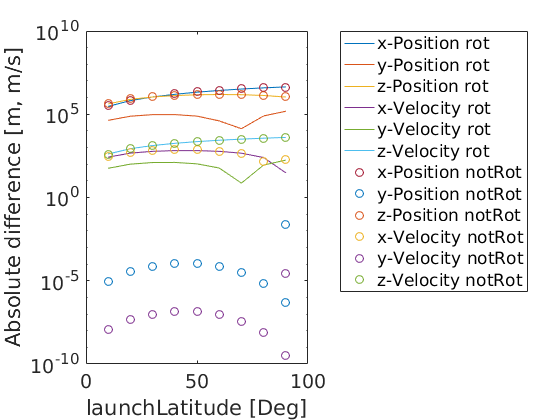
\includegraphics[width=3.1in]{figures/results/launchLatitude/launchLatitudeVsNominalAbsoluteDifferenceCase1combinedSmall.png}\label{subfig:launchLatitudeVsNominalAbsoluteDifferenceCase1combinedSmall}} 
\subfloat[]{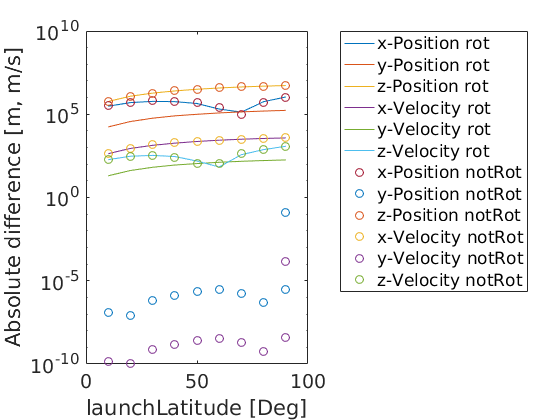
\includegraphics[width=3.1in]{figures/results/launchLatitude/launchLatitudeVsNominalAbsoluteDifferenceCase2combinedSmall.png}\label{subfig:launchLatitudeVsNominalAbsoluteDifferenceCase2combinedSmall}}
\caption{Launch latitude versus nominal absolute difference for rotating and non-rotating Mars \protect\subref{subfig:launchLatitudeVsNominalAbsoluteDifferenceCase1combinedSmall} case 1,  \protect\subref{subfig:launchLatitudeVsNominalAbsoluteDifferenceCase2combinedSmall} case 2 } 
\label{fig:launchLatitudeVsNominalAbsoluteDifferenceCase1combinedSmall} 
\end{figure} 


\begin{figure}[H]
\centering
\subfloat[]{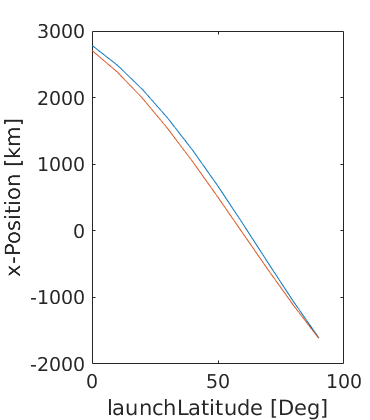
\includegraphics[scale=0.5]{figures/results/launchLatitude/launchLatitudeVsXpositionCase1combined.png}\label{subfig:launchLatitudeVsXpositionCase1combined}} 
\subfloat[]{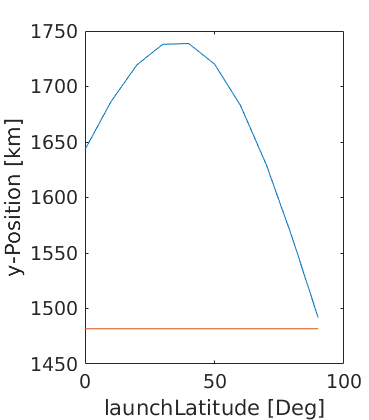
\includegraphics[scale=0.5]{figures/results/launchLatitude/launchLatitudeVsYpositionCase1combined.png}\label{subfig:launchLatitudeVsYpositionCase1combined}}
\subfloat[]{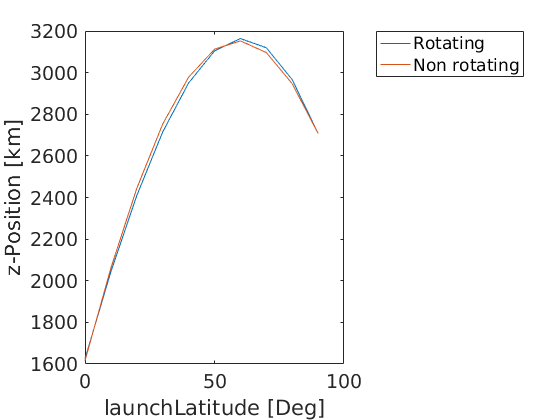
\includegraphics[scale=0.5]{figures/results/launchLatitude/launchLatitudeVsZpositionCase1combined.png}\label{subfig:launchLatitudeVsZpositionCase1combined}}\\

\subfloat[]{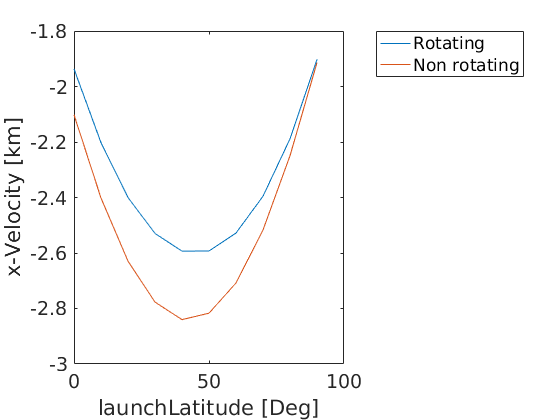
\includegraphics[scale=0.5]{figures/results/launchLatitude/launchLatitudeVsXvelocityCase1combined.png}\label{subfig:launchLatitudeVsXvelocityCase1combined}} 
\subfloat[]{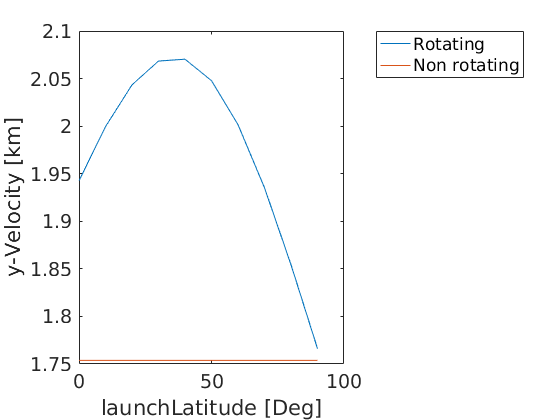
\includegraphics[scale=0.5]{figures/results/launchLatitude/launchLatitudeVsYvelocityCase1combined.png}\label{subfig:launchLatitudeVsYvelocityCase1combined}}
\subfloat[]{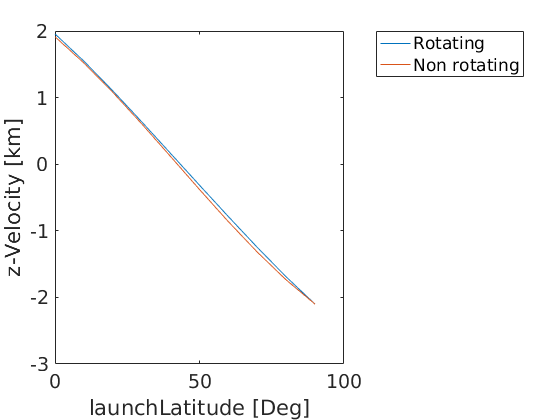
\includegraphics[scale=0.5]{figures/results/launchLatitude/launchLatitudeVsZvelocityCase1combined.png}\label{subfig:launchLatitudeVsZvelocityCase1combined}}

\caption{Launch latitude end characteristics case 1 before circularisation for rotating and non-rotating Mars \protect\subref{subfig:launchLatitudeVsXpositionCase1combined} x-position,  \protect\subref{subfig:launchLatitudeVsYpositionCase1combined} y-position,
\protect\subref{subfig:launchLatitudeVsZpositionCase1combined} z-position,  \protect\subref{subfig:launchLatitudeVsXvelocityCase1combined} x-velocity,
\protect\subref{subfig:launchLatitudeVsYvelocityCase1combined} y-velocity,  \protect\subref{subfig:launchLatitudeVsZvelocityCase1combined} z-velocity } 
\label{fig:launchLatitudeVsXpositionCase1combined} 
\end{figure} 



\begin{figure}[H]
\centering
\subfloat[]{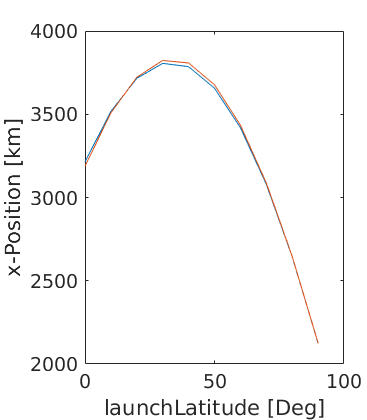
\includegraphics[scale=0.5]{figures/results/launchLatitude/launchLatitudeVsXpositionCase2combined.png}\label{subfig:launchLatitudeVsXpositionCase2combined}} 
\subfloat[]{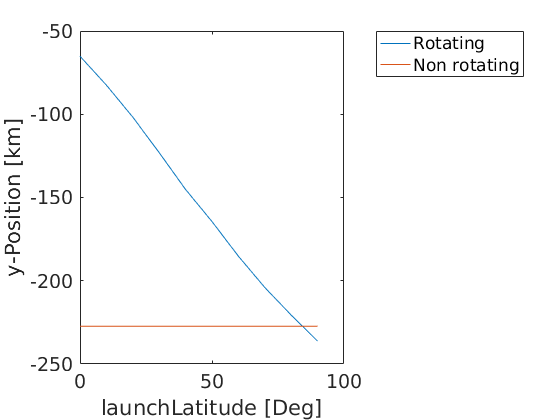
\includegraphics[scale=0.5]{figures/results/launchLatitude/launchLatitudeVsYpositionCase2combined.png}\label{subfig:launchLatitudeVsYpositionCase2combined}}
\subfloat[]{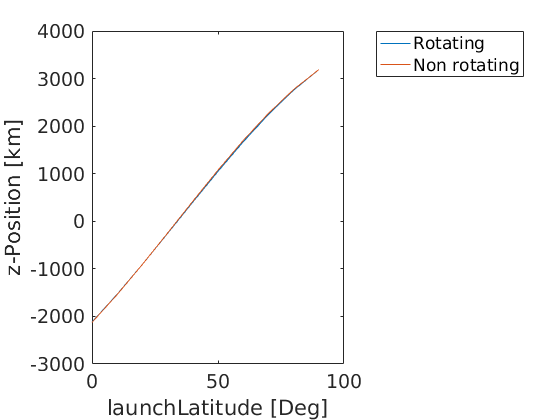
\includegraphics[scale=0.5]{figures/results/launchLatitude/launchLatitudeVsZpositionCase2combined.png}\label{subfig:launchLatitudeVsZpositionCase2combined}}\\

\subfloat[]{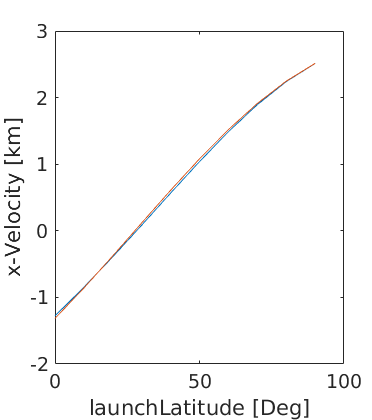
\includegraphics[scale=0.5]{figures/results/launchLatitude/launchLatitudeVsXvelocityCase2combined.png}\label{subfig:launchLatitudeVsXvelocityCase2combined}} 
\subfloat[]{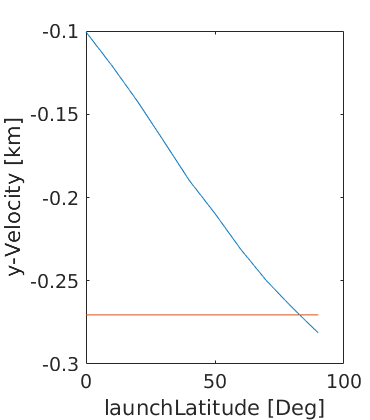
\includegraphics[scale=0.5]{figures/results/launchLatitude/launchLatitudeVsYvelocityCase2combined.png}\label{subfig:launchLatitudeVsYvelocityCase2combined}}
\subfloat[]{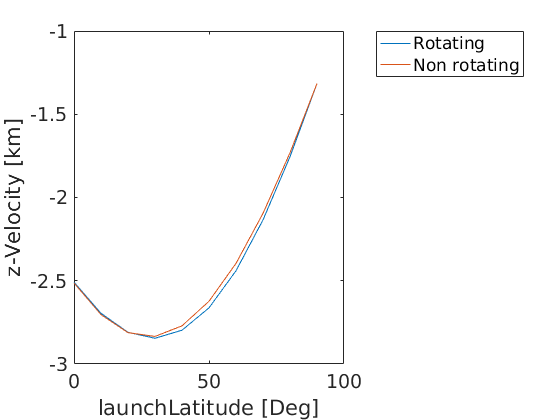
\includegraphics[scale=0.5]{figures/results/launchLatitude/launchLatitudeVsZvelocityCase2combined.png}\label{subfig:launchLatitudeVsZvelocityCase2combined}}

\caption{Launch latitude end characteristics case 2 before circularisation for rotating and non-rotating Mars \protect\subref{subfig:launchLatitudeVsXpositionCase2combined} x-position,  \protect\subref{subfig:launchLatitudeVsYpositionCase2combined} y-position,
\protect\subref{subfig:launchLatitudeVsZpositionCase2combined} z-position,  \protect\subref{subfig:launchLatitudeVsXvelocityCase2combined} x-velocity,
\protect\subref{subfig:launchLatitudeVsYvelocityCase2combined} y-velocity,  \protect\subref{subfig:launchLatitudeVsZvelocityCase2combined} z-velocity } 
\label{fig:launchLatitudeVsXpositionCase2combined} 
\end{figure} 

\begin{figure}[H]
\centering
\subfloat[]{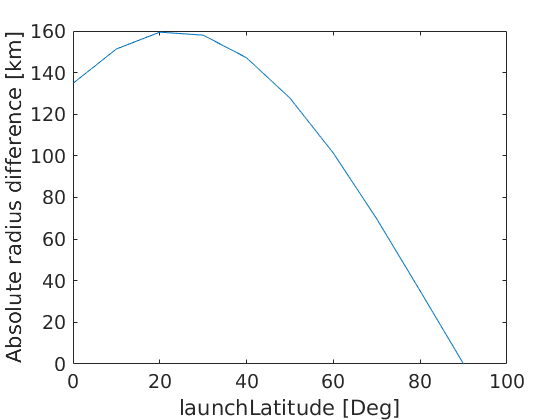
\includegraphics[width=3.1in]{figures/results/launchLatitude/launchLatitudeVsAbsRadiusDiffCase1combined.png}\label{subfig:launchLatitudeVsAbsRadiusDiffCase1combined}} 
\subfloat[]{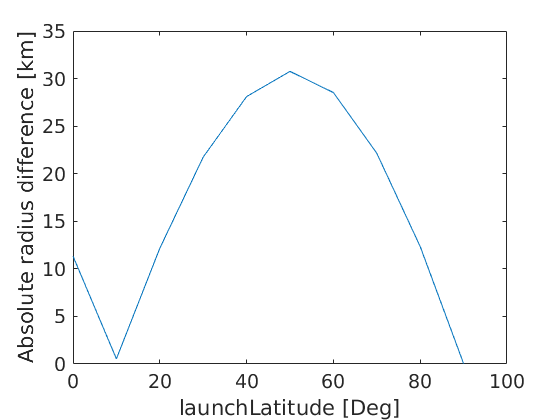
\includegraphics[width=3.1in]{figures/results/launchLatitude/launchLatitudeVsAbsRadiusDiffCase2combined.png}\label{subfig:launchLatitudeVsAbsRadiusDiffCase2combined}}
\caption{Launch latitude versus radius difference between a rotating and a non-rotating Mars \protect\subref{subfig:launchLatitudeVsAbsRadiusDiffCase1combined} case 1,  \protect\subref{subfig:launchLatitudeVsAbsRadiusDiffCase2combined} case 2 } 
\label{fig:launchLatitudeVsAbsRadiusDiffCase1combined} 
\end{figure} 

\begin{figure}[H]
\centering
\subfloat[]{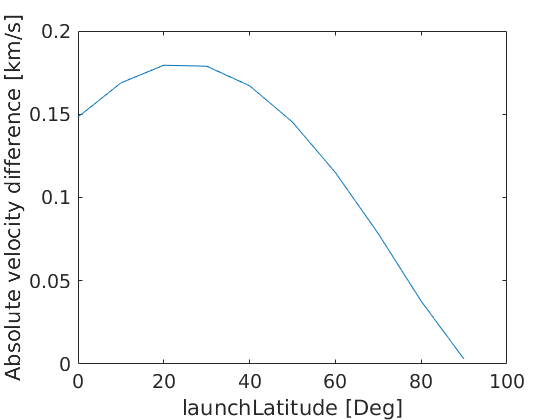
\includegraphics[width=3.1in]{figures/results/launchLatitude/launchLatitudeVsAbsVGdiffCase1combined.png}\label{subfig:launchLatitudeVsAbsVGdiffCase1combined}} 
\subfloat[]{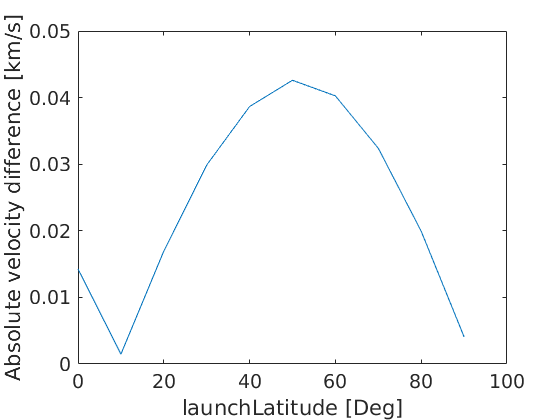
\includegraphics[width=3.1in]{figures/results/launchLatitude/launchLatitudeVsAbsVGdiffCase2combined.png}\label{subfig:launchLatitudeVsAbsVGdiffCase2combined}}
\caption{Launch latitude versus velocity difference between a rotating and a non-rotating Mars \protect\subref{subfig:launchLatitudeVsAbsVGdiffCase1combined} case 1,  \protect\subref{subfig:launchLatitudeVsAbsVGdiffCase2combined} case 2 } 
\label{fig:launchLatitudeVsAbsVGdiffCase1combined} 
\end{figure}


\section{Launch longitude}
\label{sec:launchLongitudeApp}




\begin{figure}[H]
\centering
\subfloat[]{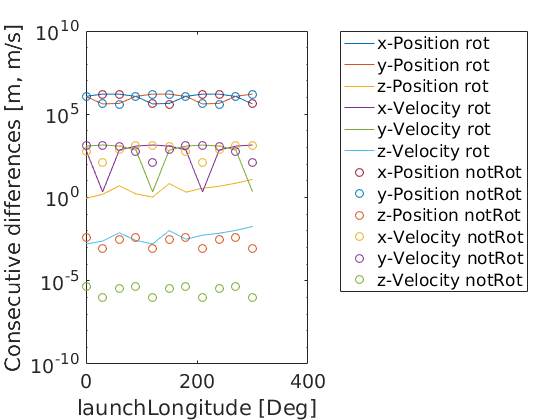
\includegraphics[width=3.1in]{figures/results/launchLongitude/launchLongitudeVsConsecutiveDifferenceCase1combinedSmall.png}\label{subfig:launchLongitudeVsConsecutiveDifferenceCase1combinedSmall}} 
\subfloat[]{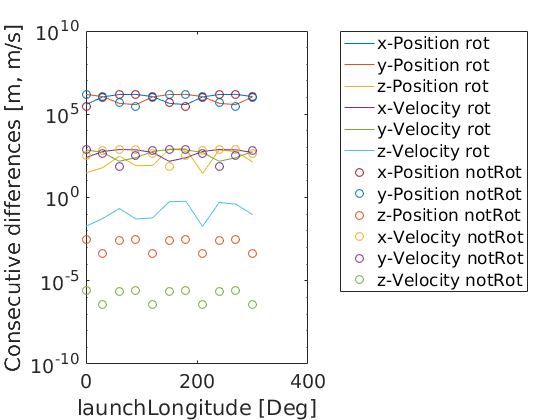
\includegraphics[width=3.1in]{figures/results/launchLongitude/launchLongitudeVsConsecutiveDifferenceCase2combinedSmall.png}\label{subfig:launchLongitudeVsConsecutiveDifferenceCase2combinedSmall}}
\caption{Launch longitude versus consecutive difference for rotating and non-rotating Mars \protect\subref{subfig:launchLongitudeVsConsecutiveDifferenceCase1combinedSmall} case 1,  \protect\subref{subfig:launchLongitudeVsConsecutiveDifferenceCase2combinedSmall} case 2 } 
\label{fig:launchLongitudeVsConsecutiveDifferenceCase1combinedSmall} 
\end{figure} 

\begin{figure}[H]
\centering
\subfloat[]{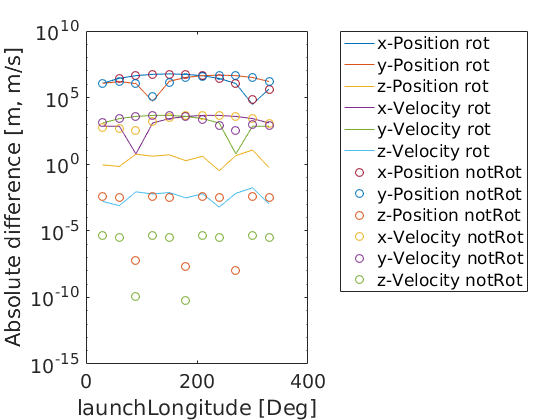
\includegraphics[width=3.1in]{figures/results/launchLongitude/launchLongitudeVsNominalAbsoluteDifferenceCase1combinedSmall.png}\label{subfig:launchLongitudeVsNominalAbsoluteDifferenceCase1combinedSmall}} 
\subfloat[]{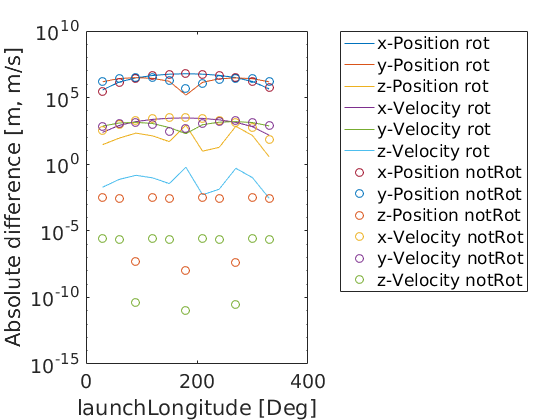
\includegraphics[width=3.1in]{figures/results/launchLongitude/launchLongitudeVsNominalAbsoluteDifferenceCase2combinedSmall.png}\label{subfig:launchLongitudeVsNominalAbsoluteDifferenceCase2combinedSmall}}
\caption{Launch longitude versus nominal absolute difference for rotating and non-rotating Mars \protect\subref{subfig:launchLongitudeVsNominalAbsoluteDifferenceCase1combinedSmall} case 1,  \protect\subref{subfig:launchLongitudeVsNominalAbsoluteDifferenceCase2combinedSmall} case 2 } 
\label{fig:launchLongitudeVsNominalAbsoluteDifferenceCase1combinedSmall} 
\end{figure}

\begin{figure}[H]
\centering
\subfloat[]{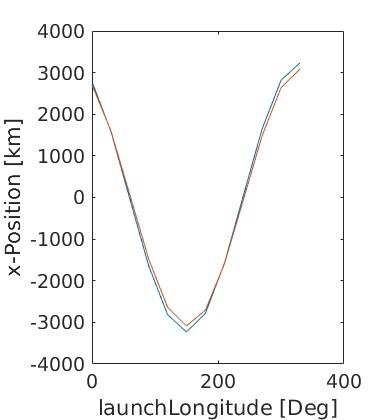
\includegraphics[scale=0.5]{figures/results/launchLongitude/launchLongitudeVsXpositionCase1combined.png}\label{subfig:launchLongitudeVsXpositionCase1combined}} 
\subfloat[]{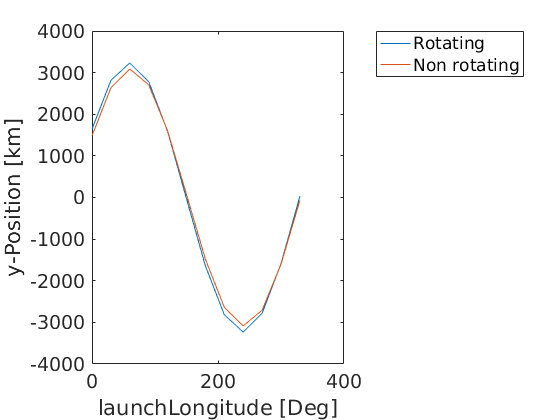
\includegraphics[scale=0.5]{figures/results/launchLongitude/launchLongitudeVsYpositionCase1combined.png}\label{subfig:launchLongitudeVsYpositionCase1combined}}
\subfloat[]{\includegraphics[scale=0.5]{figures/results/launchLongitude/launchLongitudeVsZpositionCase1combined.png}\label{subfig:launchLongitudeVsZpositionCase1combined}}\\

\subfloat[]{\includegraphics[scale=0.5]{figures/results/launchLongitude/launchLongitudeVsXvelocityCase1combined.png}\label{subfig:launchLongitudeVsXvelocityCase1combined}} 
\subfloat[]{\includegraphics[scale=0.5]{figures/results/launchLongitude/launchLongitudeVsYvelocityCase1combined.png}\label{subfig:launchLongitudeVsYvelocityCase1combined}}
\subfloat[]{\includegraphics[scale=0.5]{figures/results/launchLongitude/launchLongitudeVsZvelocityCase1combined.png}\label{subfig:launchLongitudeVsZvelocityCase1combined}}

\caption{Launch longitude end characteristics case 1 before circularisation for rotating and non-rotating Mars \protect\subref{subfig:launchLongitudeVsXpositionCase1combined} x-position,  \protect\subref{subfig:launchLongitudeVsYpositionCase1combined} y-position,
\protect\subref{subfig:launchLongitudeVsZpositionCase1combined} z-position,  \protect\subref{subfig:launchLongitudeVsXvelocityCase1combined} x-velocity,
\protect\subref{subfig:launchLongitudeVsYvelocityCase1combined} y-velocity,  \protect\subref{subfig:launchLongitudeVsZvelocityCase1combined} z-velocity } 
\label{fig:launchLongitudeVsXpositionCase1combined} 
\end{figure} 



\begin{figure}[H]
\centering
\subfloat[]{\includegraphics[scale=0.5]{figures/results/launchLongitude/launchLongitudeVsXpositionCase2combined.png}\label{subfig:launchLongitudeVsXpositionCase2combined}} 
\subfloat[]{\includegraphics[scale=0.5]{figures/results/launchLongitude/launchLongitudeVsYpositionCase2combined.png}\label{subfig:launchLongitudeVsYpositionCase2combined}}
\subfloat[]{\includegraphics[scale=0.5]{figures/results/launchLongitude/launchLongitudeVsZpositionCase2combined.png}\label{subfig:launchLongitudeVsZpositionCase2combined}}\\

\subfloat[]{\includegraphics[scale=0.5]{figures/results/launchLongitude/launchLongitudeVsXvelocityCase2combined.png}\label{subfig:launchLongitudeVsXvelocityCase2combined}} 
\subfloat[]{\includegraphics[scale=0.5]{figures/results/launchLongitude/launchLongitudeVsYvelocityCase2combined.png}\label{subfig:launchLongitudeVsYvelocityCase2combined}}
\subfloat[]{\includegraphics[scale=0.5]{figures/results/launchLongitude/launchLongitudeVsZvelocityCase2combined.png}\label{subfig:launchLongitudeVsZvelocityCase2combined}}

\caption{Launch longitude end characteristics case 2 before circularisation for rotating and non-rotating Mars \protect\subref{subfig:launchLongitudeVsXpositionCase2combined} x-position,  \protect\subref{subfig:launchLongitudeVsYpositionCase2combined} y-position,
\protect\subref{subfig:launchLongitudeVsZpositionCase2combined} z-position,  \protect\subref{subfig:launchLongitudeVsXvelocityCase2combined} x-velocity,
\protect\subref{subfig:launchLongitudeVsYvelocityCase2combined} y-velocity,  \protect\subref{subfig:launchLongitudeVsZvelocityCase2combined} z-velocity } 
\label{fig:launchLongitudeVsXpositionCase2combined} 
\end{figure} 

\begin{figure}[H]
\centering
\subfloat[]{\includegraphics[width=3.1in]{figures/results/launchLongitude/launchLongitudeVsAbsRadiusDiffCase1combined.png}\label{subfig:launchLongitudeVsAbsRadiusDiffCase1combined}} 
\subfloat[]{\includegraphics[width=3.1in]{figures/results/launchLongitude/launchLongitudeVsAbsRadiusDiffCase2combined.png}\label{subfig:launchLongitudeVsAbsRadiusDiffCase2combined}}
\caption{Launch longitude versus radius difference between a rotating and a non-rotating Mars \protect\subref{subfig:launchLongitudeVsAbsRadiusDiffCase1combined} case 1,  \protect\subref{subfig:launchLongitudeVsAbsRadiusDiffCase2combined} case 2 } 
\label{fig:launchLongitudeVsAbsRadiusDiffCase1combined} 
\end{figure} 

\begin{figure}[H]
\centering
\subfloat[]{\includegraphics[width=3.1in]{figures/results/launchLongitude/launchLongitudeVsAbsVGdiffCase1combined.png}\label{subfig:launchLongitudeVsAbsVGdiffCase1combined}} 
\subfloat[]{\includegraphics[width=3.1in]{figures/results/launchLongitude/launchLongitudeVsAbsVGdiffCase2combined.png}\label{subfig:launchLongitudeVsAbsVGdiffCase2combined}}
\caption{Launch longitude versus velocity difference between a rotating and a non-rotating Mars \protect\subref{subfig:launchLongitudeVsAbsVGdiffCase1combined} case 1,  \protect\subref{subfig:launchLongitudeVsAbsVGdiffCase2combined} case 2 } 
\label{fig:launchLongitudeVsAbsVGdiffCase1combined} 
\end{figure}

%\section{Flight-path angle}
%\label{sec:flightPathAngleApp}
%
%\section{Heading angle}
%\label{sec:headingAngleApp}